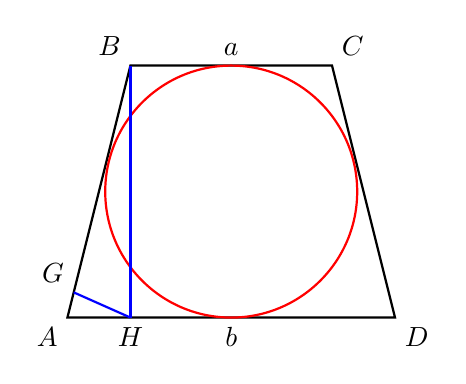
\begin{tikzpicture}[scale=0.8]
    \coordinate (A) at (0, 0);
    \coordinate (B) at (1, 4);
    \coordinate (C) at (4.2, 4);
    \coordinate (D) at (5.2, 0);
    
    \coordinate (G) at (0.1, 0.4);
    \coordinate (H) at (1, 0);
    
    \draw [thick] (A) -- (B) -- (C) -- (D) -- cycle;
    
    \draw [red, thick] (2.6, 2) circle [radius=2];

    \draw [blue, thick] (B) -- (H);
    \draw [blue, thick] (G) -- (H);

    \node [below left] at (A) {\( A \)};
    \node [above left] at (B) {\( B \)};
    \node [above right] at (C) {\( C \)};
    \node [below right] at (D) {\( D \)};
    
    \node [below] at (H) {\( H \)};
    \node [above left] at (G) {\( G \)};
    
    \node [above] at (2.6, 4) {\( a \)};
    \node [below] at (2.6, 0) {\( b \)};
\end{tikzpicture}